\chapter{Head To Toe 4}

% \begin{figure}[H]
%     \centering
%     \includegraphics[width=\textwidth/2]{./Games/EveryChildCanSucceed/Images/EveryChildCanSucceed1CD.png}
%     \caption{Every Child Can Succeed 1 CD}
% \end{figure}

The final of the Head To Toe games published and released by The Lightspan Partnership for the PlayStation 1.

Head To Toe 4 features three video programs:

\begin{itemize}
    \item A Healthy Smile
    \item Staying Healthy
    \item Safety First
\end{itemize}

\clearpage
\newpage

\section{A Healthy Smile}

\subsection{Audio Summary}

"A Healthy Smile" describes how and why children lose their baby teeth, and what they can do to keep their teeth healthy.

\subsection{Transcription}

Bob: Okay everybody, hold still. Smile. Uh, wait a minute, something's missing.

Arnell: Everybody's here.

Bob: No that's not what I mean, Arnell. Something else is missing, something in Jody's mouth. Did you lose something yesterday?

Jody: Oh, my tooth!

Bob: What happened to it?

Jody: It just fell out.

Bob: Wow, that's kind of neat. It looks like you've lost more than one though.

Jody: Yes, I've lost other ones.

Arnell: Yeah, I lost some too.

Bob: You have Arnell?

Arnell: Eight of them.

Bob: Wow, have you lost any teeth recently?

Naomi: Bob, why do we lose our baby teeth?

Bob: That's a very good question, Naomi. Maybe that's why today's a good day to think about our teeth.

(video plays)

Bob (voice over): You probably know that your first set of teeth don't last very long. We sometimes call them your baby teeth. Somewhere around the age of five or six or seven, you begin to lose your baby teeth one at a time. That's good because they're being pushed out by new bigger, stronger teeth. We call those new teeth your permanent teeth or your adult teeth.

(back to the house)

Bob: I can show you why that happens. This is a model of baby teeth. Now Jody can already see that these teeth are loose and they're coming out, but what she cannot see is what's happening behind this pink skin that we call the gums. Behind that, there's another row of teeth. These are the baby teeth, and below and above them are the permanent teeth. Now let's just look at the top row. Here are the baby teeth, and here are the permanent teeth. Now they're pretty small right now, but as they grow and get bigger, they push the baby teeth out. So eventually, one by one, all the baby teeth are replaced with a set of permanent teeth. And these are called permanent teeth because if you take care of them, you have them for the rest of your life. An-

Arnell: Bob!

Bob: Arnell, what?

Arnell: Jody's permanent teeth have already grown in!

Bob: Already?

Arnell: Uh-huh. Look!

Bob: Whoa, boy! You must have a hard time brushing those teeth. Yeah, you wise guys. Somehow I feel that those were not really Jody's permanent teeth. But it did get me thinking, do you brush your teeth? I'm sure people have told you that if you don't brush your teeth, you're going to get cavities. But have you ever wondered what makes cavities? You might be surprised. Let me show you.

(moves to the next room)

Bob: Have you ever heard the word acid? This is how you spell it: A-C-I-D. Acid. Now, do you know what acids are? Well there are lots of different kinds of acids, but some of them can actually eat away or burn other materials. Let me show you what a little bit of acid can do. This is a piece of limestone, and it's very hard material. And this is a very powerful acid. In fact, this acid is so strong that I have to protect my skin, so I have to wear some gloves so that it won't get on my skin. This acid is stronger than any acid you'd have at home in your school, so you'd never do this kind of experiment yourself. I also have to protect my eyes because I don't want any of this acid to splash into my face. Now watch what happens when I just take a few drops in this eyedropper of this acid and put it on the limestone. So we'll just get a few drops drawn up in here, and watch what they do. And look at how that acid eats away at that very hard limestone. It's also turning it brown. And if I was to keep doing that, eventually that acid would eat right through that piece of limestone. Here's a piece that we put some acid on earlier, and you can see how it's eaten it away. It turned it really brown like that, and there's a big depression here. And see there, it's almost all the way through that very hard stuff. This is stone, and the acid ate its way right through it. Well, your teeth, the covering on the outside of your teeth, the white part, is very hard material. In fact, it's the hardest material in your body, and you want to take care of that so that you'll have your teeth for the rest of your life. But cavities are holes in that hard outer covering. Here's one here, and there's another one there, and you can see how they're brown and they've gone right through that hard covering. Now, what can make those holes in the covering of your teeth? Well, you've probably already guessed: acids. You have acids in your mouth, and they eat away at your teeth and make holes in them. Now you're probably saying to yourself, 'wait a minute, I don't eat acid. I mean, I eat fruits, I eat vegetables, I eat yogurt, I eat meat. I wouldn't put a dangerous chemical like that in my mouth.' And you never should put a chemical like that in your mouth because it is very dangerous. So how do you get cavities? Well, something happens to the food that you put in your mouth.

(video plays)

Bob (voice over): After you chew your food, you swallow most of it. But some food is always left in your mouth along the gums and in the spaces between your teeth. A lot of food has sugar in it. When it mixes with the liquids in your mouth, it turns into\dots acid! And that acid can start to make tiny holes in your teeth. And before you know it, ouch! You have cavities.

(back to the house)

Bob: So sugary food left in your mouth turns into acid. So if you don't want cavities, you have to clean that food away. And it looks like Tiffany has the best way to do that.

Tiffany: That brush your teeth.

Bob: Exactly. And how often should you brush your teeth, Tiffany?

Tiffany: After every meal and before you go to bed.

Bob: Right. Now, brushing your teeth is important, but so is how you brush your teeth. Tiffany, would you like to show us how to do that?

Tiffany: Okay.

Bob: I'll be the mouth.

Tiffany: You should always brush up and down in the direction that your teeth grow. You may open up, Bob.

Bob: Eugh.

Tiffany: And do the same on the inside. And don't forget the tops. You may close now, Bob. It's also important to brush your gums. It helps to keep them healthy.

Bob: That's great, Tiffany. Thank you. If you brush your teeth like that after every meal and before you go to bed, you will wash away that leftover food, and you'll have fewer cavities. But is brushing your teeth enough? Does it get all of the food? Well, recently Christopher learned a whole lot about that.

(video plays)

Dentist: Looks good. You're doing a good job brushing, keep it up. Just going to make sure we don't have any hard deposits down here, that tartar, that calculus. Let's check up here, right up along here. I want you to get that toothbrush up along your gums and brush your teeth and your gums real gentle there on the outside and on the inside there. Good job. No cavities, that's what we like. You come in here every six months with no cavities, that's good. You ready to get them cleaned? Shine them up for you.

(skip forward to the cleaning)

Dentist: You're doing super. Wish everybody was as good a brusher as you.

(skip forward to the fluoride treatment)

Dentist: Okay, we're going to do your fluoride treatment now. Are you ready?

Christopher: Yep.

Dentist: Okay, going to have you take half of that in your mouth. I want you to swish it around. Good job. I'll take that. I'm going to time you for one minute. Then we'll let you spit into the [sweetner]. Okay, swish it in and out between your teeth, that's important.

(skip forward to the end of the visit)

Dentist: Okay, we're done with the fluoride, you're done with your cleaning. No cavities, that's good. Going to send you home with a new toothbrush. Want you use it every day, at least twice a day. Good.

Christopher: Okay, thank you.

Dentist: You're welcome. How about a prize or a sticker or something?

Christopher: Yeah, okay.

Dentist: Alright.

(new video plays)

Female Singer 1: You brushed in the front, you brushed in the back. You brushed every night before bed. So you were feeling confident when the dentist took a look, but boy were you surprised when the dentist said you have two cavities.

Female Singer 2: Two cavities!

Female Singer 1: I found two cavities.

Female Singer 2: Two cavities! The news was very hard to take. I yelled, 'There must be some mistake!' When the dentist said -

Female Singer 1: You have two cavities.

Female Singer 2: I brushed in the front, I brushed in the back. I brushed after every single meal. I even take my toothbrush to school every day, so this cavity thing just can't be real.

Female Singer 1: You have two cavities.

Female Singer 2: Two cavities.

Female Singer 1: You have two cavities.

Female Singer 2: Two cavities.

Female Singer 1: Am I getting my point across? You really also have to floss. It's a shame, but you have two cavities.

Female Singer 2: Floss, just floss and you will see, a great big smile in the dentist's -

Main: Ah, I found no cavities!

Female Singer 2: Now you floss in the front, and you floss in the back. The dentist got her point across. And I haven't had a cavity in two whole years.

Female Singer 1: No she hasn't had a cavity in two whole years.

Both Female Singers: There hasn't been a cavity in two whole years.

Female Singer 2: Just because I know how to floss.

(Back to the house)

Bob: So brushing and flossing and getting a regular checkup, all of these keep your teeth clean on the outside. But you can also keep your teeth healthy and strong from the inside. Right, Arnell?

(video plays)

Arnell: Hi, do you know which food is best for your teeth? Let's see. What drink is best for your teeth: soda, milk, or orange juice? You have 5 seconds. Bzz! Time's up! What did you pick? The answer is milk. Anything made out of milk makes your teeth strong and healthy. Remember that. Now, which one of these foods is good for your teeth: candy, bread, or cheese? The candy thing we can get rid of right away 'cause everybody knows candy is not good for your teeth. So bread or cheese? You have 5 seconds. Bzz! Time's up! The correct answer is cheese. Did you get that? I told you that anything that was made from milk was good for your teeth, and cheese is made from milk. One more. Which one of these is good for your teeth: buttermilk or yogurt? Warning: this is a trick question. You have 5 seconds. But time's up! The answer is both of them. Alright!

(next video plays)

Bob (voice over): Your baby teeth are soon replaced by permanent teeth. The covering on your teeth is the hardest part of your body, but sugar and food left in your teeth turns into acid and causes cavities. The best way to get rid of that food is to brush after every meal and before bed. And to clean the spaces between your teeth, you should floss every day. A checkup every 6 months will keep your teeth clean and healthy, and you'll catch any small cavities before they turn into big ones. To strengthen your teeth from the inside, drink milk and eat cheese and yogurt.

(back to the house)

Bob: Boy, isn't it great that a delicious tasting food like ice cream is also good for you?

Jody: Good for your teeth

Tiffany: Because it's made with milk.

Bob: What do you think about all this, Arnell?

Arnell: I say this is something you can sink your teeth into.

Jody: Yeah!

Bob: Right! Now wait a minute, before you eat, I still haven't got my picture of you guys. So all right, everybody\dots Ice cream!

\subsection{Credits}

Models Donated by: Frey Scientific Inc, Denoyer-Geppert Science Company;
Special Thanks to: Julie Panyard (Dental Health Educator);

\section{Staying Healthy}

\subsection{Audio Summary}

"Staying Healthy" shows children making healthy choices in the things they eat, the way they behave, and the games they play.

\subsection{Transcription}

Bob: You know who this is? It's Arnell when he was only 6 months old.

Arnell: I was a cute kid.

Bob: And here's another cute kid. This is a picture of Louisa.

Louisa: I was only one year old.

Bob: And this baby's even younger. It's a picture of Sarah when she was only a few months old.

Sarah: I already had a lot of hair.

Bob: Do any of you remember being that little?

Children Together: No.

Bob: Ah now, you know it wasn't that long ago since you were a baby and you couldn't do very much back then. Adults had to do almost everything for you. They had to feed you and clothe you and keep you warm. But now you can do all of those things by yourself, and that's what we want to talk about today: how you've become bigger and stronger and faster and more wonderful a-

Arnell: And more wonderful!

Bob: Yeah, and more wonderful, come here, clown! Every day. You know when you think about all of the things that you can do, you really see just how much you've learned since you were born. Right?

Arnell: Yep!

(move to the next room)

Bob: Here's something that you might have used when you were a little kid, right? This was probably the most important toy to you in the whole world when you were a baby. Do you use rattles now?

Children Together: No.

Sarah: No way!

Bob: You don't play with rattles now. What kind of toys do you play with now? What do you like?

Louisa: Books!

Bob: Books, yeah sure. You like to read books. I like to read books too. Here, a nice storybook there. What else? What else you like to read? Hey?

Arnell: Dinosaur!

Bob: Dinosaur! Sure, I just happen to have a dinosaur right there. Yeah, what else?

Sarah: Building set!

Bob: Building sets? Well, I just happen to have a building set right there. Sure, go build yourself a bridge.

Louisa: Jump rope!

Bob: Jump rope! Yeah, that's a lot of fun. Yeah, good exercise there on the jump rope. There you are Louisa.

Arnell: Cards!

Bob: Cards? Oh, you want to have a game of cards? I think I got some. Oh, there's a game of cards.

Sarah: Checkers!

Bob: Checkers, that's something that I like to play. You know, I like to play games. I like to play games like checkers, and here's another one that I'm still learning. I'm not very good at this one. This one's called the ball in a cup. You have to try to get the ball to stay in the cup like that, except you can't put it there with your hand. You have to do it like this. Watch. Oh, almost had it. Yeah, I'm not very good at that. I'm still trying to learn it. Maybe you like to make up some games by yourself, or maybe you like to play one of these things, hm? I know Arnell likes to play computer games. Yeah, they're a lot of fun. But isn't there a big difference between this computer game and this rattle? You didn't play computer games when you were a baby. Now you can because you're bigger and you're smarter.

(video plays)

Louisa: This is Berkley. She's a cat. My mom said I could have a cat only if I took care of her myself. So that means I got to feed Berkley, make sure she gets water, clean out her box. That's my job. I do it everyday. Say hi, Berkley!

Louisa (pretending to be a cat): Hi, everybody!

Louisa: I'm surprised that I take such good care of Berkley.

(skip to Arnell)

Arnell: I draw pictures mostly with my crayons or chalk. But for my birthday, I got a bunch of markers, and this is what I did with them. I'm very proud that I made this picture because this is someplace that I made up. It has three suns and people with green hair. Oh, and you can see that ping pong balls grow out of the trees. Even though this is a made-up place, I would still like to go here someday.

(skip to Sarah)

Sarah: I do gymnastics. I used to just do it myself, like doing cartwheels in the park, but now I go to gymnastics class, and we're learning tumbling and handstands, and my favorite thing, which is sort of like dancing and tumbling at the same time. Oh, and we had a gymnastics meet and I was in it and I got a ribbon. I'm proud that I can do gymnastics.

(back to the house)

Bob: Drawing, taking care of a pet, gymnastics - these are all things that you can do now. Almost had it! And you're learning to do new things every day. So you can do a lot. In fact, if we were to make a list of all of the things that you can do, it would probably be quite long. Let's watch.

(video plays)

Girl (singing): When I was a baby, I didn't do much except eat and sleep and cry. Now that I'm older, I do lots of things. Did you know that I can, I can, whistle a tune, draw a cartoon, look at the moon, and use a spoon? And maybe someday soon, I'll fly in a balloon. I can turn out the light, read and write, be polite, and stay overnight. And tomorrow I just might go fly a kite.

Backing vocals: I can, I can, I can, I can, I can, I can, I can, I can.

Girl (singing): I can take a hike, ride my bike, hit a ball, stand real tall, tie my shoes, pick and choose. I can hardly wait to hear what I can do next year.

(back to the house)

Bob: Yes, you can do a lot of things all by yourself. But that means that you get to make choices. Maybe you choose what you do when you come home from school. You might choose what you're going to eat at a restaurant. I know you choose what toys you're going to play with. I've chosen this one, even though I'm not very good at it. And many of the choices that you make every day affect your health. But do you make healthy choices? Let's see. When you come home for lunch, do you run right to the table and start eating, or do you wash your hands first? Which is the healthier choice? After you finish lunch, do you run right out and jump on your bike to go for a ride, or do you brush your teeth first? Which choice is better for your body? Look at this great tree. It'd be fun to climb all the way to the top, but it's very high and it could be dangerous. So do you climb right up, or do you wait until a parent or an adult tells you that it's okay to go that high? You can make these decisions, and you can do it. Just like you can ride a bicycle or turn a somersault, you can make the decisions that are best for your health. In fact, that's what growing up is all about: making healthy choices. Here's one more: Arnell and Joy and their dad went camping. They had some choices to make. Did they make healthy choices? Let's see.

(video plays)

Bob (voice over): Joy and Arnell love to go camping with their dad. This time their friend Chao came along too.

Dad: Do you guys know how to put up this tent?

Chao: Of course. I do it all the time.

Dad: Are you sure you know how to put up this tent?

Chao: Yeah!

Arnell: No, but we can figure it out.

Dad: Well, if you need help, just ask me.

Joy: Hey, what's this doing here?

Chao: Hey, get me out of here!

Joy: Are you okay? I didn't mean to.

Arnell: Yeah, she didn't mean to.

Joy: Maybe we should ask Dad to help us.

Chao: No, I want to do it myself.

Joy: We might even break it.

Arnell: But right now it's too hard.

Bob (voice over): The kids have to make a choice.

Chao: Okay.

Arnell: Dad, we need some help!

Dad: All right, I'm coming.

Bob (voice over): Asking for help when you need it is always a good choice.

(skip forward to the tent being put up)

Joy: We did it!

Chao: Cha-ching!

Dad: Right. Hey, we're a good team. What do you say if I get everybody something to drink?

Kids: Yeah!

Dad: All right, come on. Let's get it. All right, let's see what we have here. Okay, we got fruit juice, we got soda, and we got some water.

Bob (voice over): What would be a healthy choice?

Arnell: I'll take fruit juice.

Dad: Okay, there you go.

Joy: I'll take water.

Dad: Water, all right.

Chao: Juice for me, please.

Dad: Juice for you too. Okay.

Bob (voice over): That's the healthy idea.

(skip forward in the video)

Dad: Hey, who's going to help me make lunch?

Bob (voice over): Chao is having fun all by himself, but he has to make a choice.

Chao: I'm coming!

Bob (voice over): Doing your part when there's work to be done: that's a great choice.

(skip forward in the video)

Dad: Hey, you guys hurry up over there. It's time to eat. Wash your hands real good now. All right, good, good, good, good.

Chao: What can we do after lunch today?

Dad: Well, there's a lot of things we can do out here: we can take a hike or maybe it'd be fun to even go fishing.

Arnell: I want to do everything!

Dad: Well, we can try.

Arnell: Yes!

(skip forward in the video)

Joy: Yes, look at that [inaudible] tree! I like [inaudible].

Dad: Yeah, it's going to be big one day. Real big.

Arnell: Hey, look at that groundhog!

Chao: Cool!

Arnell: Let's go see where it goes!

Chao: No!

Arnell: Hurry up or we'll lose it!

Bob (voice over): It would be fun to see where that groundhog lives, but Chao and Arnell have to make a choice.

Chao: Arnell! Your dad told us to stay close; to be safe. Arnell!

Arnell: Yeah, you're right. But I bet you I can beat you to 'em!

(skip forward in the video)

Arnell: I don't get fishing.

Dad: What do you mean?

Arnell: Nothing ever happens.

Dad: Well, you have to be patient.

Arnell: Woah, I think I've got something!

Joy: What is it?

Arnell: It's gigantic! It's a shark! It's a very, very big shark!

Chao: It's a bucket! It's a bucket shark! Very dangerous.

Dad: Nice fish.

(back to the house)

Bob: So what happened then?

Arnell: Well, we made a campfire, we roasted marshmallows, and we told ghost stories.

Bob: Ghost stories? Boy, you had a pretty good time on that trip, didn't you?

Arnell: Yeah.

Bob: Well\dots Listen, let's take this, um, shark, looks like a scary one, and let's put it over here someplace special. Come on. It's good to save things that you're proud of, things that remind you of good times or when you did good things. So we're going to put your bucket shark up here on the shelf. Okay?

(video plays)

Bob (voice over): When you were a baby, you couldn't do very much. Now you're learning all kinds of new things. You're proud of the things you can do. Now that you can do a lot of things, you have to make choices. It's up to you to make the choices that will keep you healthy, healthy and strong.

(back to the house)

Bob: Can you guess who this is? It's me! Yes, they did have cameras back then. I can do a lot of things now that I couldn't do then. I can drive a car, I can sail a boat, I can play guitar - lots of things that I've learned to do. And you know something else? I'm still learning new things every day.

Children Together: Yay!

Bob: What do you think? Okay, you try it. See if you can get it on the first time. That was pretty good! I got it right the first time! Oh, I guess I got lucky.

\subsection{Credits}

Special Thanks to: [Merrill and Lorene Scolt Farm];
Models Donated by: Frey Scientific Inc, Denoyer-Geppert Science Company;

\section{Safety First}

\subsection{Audio Summary}

"Safety First" talks about how to keep safe in the home and elsewhere, the use of safety devices, phoning 911, and personal responsibility.

\subsection{Transcription}

Sam: Some things in your house are waiting to get you. Wooo!

Chao: They're in the kitchen.

Sam: They're in every room. Wooo!

Bob: You might not even be safe even in your own bedroom! And that's because\dots

Naomi: Lots of things can get you if you don't watch out.

All Together: Wooo!

Bob: Christopher knows. Watch.

All Together: Wooo!

(video plays)

Christopher: I'm standing in front of one of the most dangerous places on Earth. This is where they keep poison and sharp knives and explosives and mysterious drugs. Scary, huh? Today I'm going in this dangerous place. Why? Because I live here. Come on!

(enters his house)

Christopher: Mom, I'm home!

Christopher's Mom: Hi Chris, I'll see you in just a minute.

Christopher: You know what? Every year more kids get hurt at home than any place else. It's true. That's because we like to play, and some of the things we play with are really dangerous. I'll show you some of the things in my house that are dangerous.

(enters the living room)

Christopher: My dad goes hunting, so he keeps his guns in the house. They're usually locked up, but sometimes the doors open. I could play with the guns if I really wanted to, but I'd never do that because I know that thousands of kids every year get hurt from playing with real guns. Some of them even get killed. There's one more thing. There's something in every single room that can burn you. It's not fire, but still, it can burn you really bad: up there and over there

(moves to another room)

Christopher: Earthlectricity. It's everywhere in your house, but that doesn't mean it's safe. Never put anything into a wall socket or in a light. That means your fingers or a pen or a toy or anything. And if you ever see sparks or smoke, run and tell your parents. Electricity is not a toy.

(moves to the kitchen)

Christopher: You think that's scary? This place is even worse: the kitchen. First of all, look at all these knives. They are definitely sharp, and they could definitely cut your skin wide open. Never use a knife unless a grownup is with you. Second of all, look down here. What's in all these bottles and cans? I'll tell you what: poison. If you swallow it, they might have to take you to the hospital, and some of it hurts if you just get it on your skin. I'm telling you, stay out of here. Under the sink is definitely a grownup place. And so is this: medicine. When you're sick, it might be good for you, but if you swallow medicine that's for somebody else, it can make you sick. Let your parents give you medicine when you need it.

(moves to the shed)

Christopher: Tools can be really handy, but if you don't use them right, they can also be dangerous. So never use a tool unless a grown-up is with you.

(moves to the front of the house)

Christopher: There are a lot of things that can get me in my house, but I'm not scared. Because if you know what to play with and what not to play with, you'll be safe at home.

(back to the house)

Bob: *blowing out candle smoke from a fire alarm* Whew.

Naomi: That's loud!

Bob: Yeah, well it's supposed to be loud so that you'll hear it whenever there's a fire. A smoke alarm can save your life. Oh, somebody at the door. Here, just a minute.

Paula: Hi Bob! Hi kids! Listen, I just passed by and heard the smoke alarm. Is everything okay?

Bob: Oh, oh yeah, yeah, it's okay. We were, we were just testing it and we're actually, we're talking about safety.

Paula: Safety?

Bob: Yeah.

Paula: I just happened to know a song about safety. Would you like to hear it?

Bob: Come on, you don't have a song about safety.

Paula: Yeah!

Bob: Well, come on. Yeah, come on, we'd like to hear it.

Paula: Come on.

(move to another room)

Paula: Actually, I've been singing this song quite a bit to my new baby.

Bob: Sam, come on in! Paula's got a song about safety.

Sam: Hi Paula!

Paula: Hi Sam! Guess what? I brought my own music too.

Bob: Really?

Chao: You did?

Bob: How'd you do that?

Paula (singing): It's okay to play, it's okay to have fun, and secrets are okay too. But you really got to think about what you're playing with and what you're playing with could do. So if you aren't really sure or you just don't know, I've got something to share with you. Just play it smart, just play it safe, 'cause you don't want an ouchie or a bandage or a big black and blue boo-boo. Play it safe if you don't know what it is, play it safe, just leave it alone. Play it safe if you don't know what it'll do, play it safe, just leave it alone. Play it safe, and before you play, find out what it is and if it's okay. Play it safe, just leave it alone, and you'll be safe at home.

Everyone Together: Play it safe if you don't know what it is, play it safe, just leave it alone. Play it safe if you don't know what it'll do, play it safe, just leave it alone. Play it safe, and before you play, find out what it is and if it's okay. Play it safe, just leave it alone, and you'll be safe at home.

Bob: Wow, great song, Paula!

Paula: Thanks! Oh, look at the time, I've got to go. Bye bye!

Children Together: Bye bye!

Bob: Bye Paula!

Chao: Bye!

Bob: Wow, wasn't that a great song on safety?

Children Together: Yeah!

Chao: Yeah, that was great!

Bob: Wow! And wasn't it scary how Paula just happened to know a song about safety just as we were talking about a smoke alarm?

Everyone Together: Ooooh!

Bob: But you know, it is important to talk about safety and smoke alarms and fire. For example, what do you think the first thing is that you should do if there's a fire in your house? Should you try to put the fire out yourself? Should you get out of the house? Should you try to grab all your toys and things and try to save them? You decide. And the correct answer is:

Chao: Get out of the house!

Bob: As quickly as possible. Don't try to put the fire out yourself because that's a very difficult thing to do, and you might actually make it worse. And don't try to save anything because the most valuable thing in the house is you. Your parents and your friends want you to be safe too, so meet them outside, or if there's nobody around, go to a neighbor. Now suppose you wake up in the middle of the night and your bedroom is completely filled with smoke, and there's so much smoke that you can't see anything. Do you know what to do? Do you know, Naomi?

Naomi: Yes.

Bob: Can you show us?

Naomi: Sure. *cough cough* Oh no, the room's all full with smoke! I can't see anything!

Bob: Great! Did you see what she did? She got down on her hands and knees and crawled out of the room. Good stuff, Naomi! And that's what you should do because smoke always rises to the top of the room first. So if this room actually was filled with smoke, it may only come down to about here. Down here, there may not be any smoke at all, so you can not only breathe better, but you can see better as well.

Naomi: I know something else.

Bob: What's that?

Naomi: I know what to do if our clothes ever catch on fire.

Sam: I do too!

Chao: So do I!

Bob: Okay. Then why don't you all tell us what to do when your clothes are on fire?

Naomi: Stop.

Chao: Drop.

Sam: And roll!

Bob: Bravo, bravo! Just think: stop, drop, and roll. Don't try to run because that might make the fire worse. So stop what you're doing, then drop to the ground and roll around. And that's the best thing to do if your clothes ever catch on fire. So what is it, kids?

Everyone Together: Stop, drop, and roll!

(video plays)

Bob: Going places is a lot of fun, but you have to be careful when you're not at home because you can hurt yourself in a lot of different ways. Sam and Chao and Naomi can show us some of the things that they do to be safe when they're not at home.

Sam: There are lots of things you can do to make bike riding safer, like this book bag. If I didn't have a book bag and I had to carry some books home from school, I could only ride with one hand. And that's not only dangerous, it's stupid! You should always ride with both hands. And I have reflectors: I have one on the front and one on the back and one on both wheels. And I have a light in case I'm ever out riding with my parents and it gets dark. I want cars to be able to see me and hear me. But do you know the thing on my bike that makes it really, really safe? Me! I make my bike safe, because I know how to ride safely.

(next scene in the video)

Sam (voice over): I always ride on the right side of the road. I stop at stop signs and, of course, at red lights.

(next scene in the video)

Sam (voice over): This isn't very smart. See, when we ride side by side, we take up almost the whole street. Then cars can't get by. This is much better. Now cars can get by. Do you know the hand signals for turning? This means I'm turning right. This means I'm turning left.

(next scene in the video)

Naomi (voice over): I walk places every day. When I cross the street, I always cross at the corner. If there's a crosswalk, I cross the street there. A crosswalk looks like this.

(next scene in the video)

Chao: Let's go for a ride in the car. Wait, I'm not safe yet! Now I'm safe. Let's go!

(back to the house)

Bob: You know the great thing about Chao wearing his seat belt or Sam riding her bike safely or Naomi looking both ways before she crosses the street? They're kids just like you, and they've taken responsibility for their own safety. You know, that's an important part of growing up, is learning how to take care of yourself. And you can do that - you can make safe choices every day. Now let me give you an example: suppose a stranger, somebody you don't know, starts talking to you. Suppose this stranger wants to give you something or take you for a ride in their car. What should you do? Well, why don't you take responsibility and find out? Ask your teacher or ask your parents what you should do if a stranger talks to you. You can do it. You can find out what's safe, and that's important.

(video plays)

Bob (voice over): Your home can be a dangerous place. Grown-up things like guns and knives, cleaning materials, and medicine - these are not toys. They can hurt you. Electricity is dangerous too. If your house is on fire, the best thing to do is to get out as fast as you can. If there's a lot of smoke, crawl on the ground. If your clothes catch fire, remember: stop, drop, and roll. Learn how to make your bike safe. Always obey street signs and traffic lights and ride single file so cars can pass. When you go walking, always look both ways before you cross. Cross the street at the corner. Look for a traffic light or a crosswalk. Fasten your seat belt when you go for a ride in a car.

(back to the house)

Bob: One more thing: if you are in any kind of trouble, get to a telephone and remember this number: 911. That's the number of the people who can help you. 911. If you're in a fire, if somebody's really sick, or if you're in any kind of trouble at all, dial 911 and have someone show you where those numbers are on the telephone.

Children Together: Bob! Bob! Bob!

Bob: What, what, what?

Sam: We have a question.

Bob: Okay, sit down. Let's talk about it. Come right in here. Okay, what's up?

Sam: Well, if you get lost like at the mall or in a park, what should you do?

Naomi: Stand still.

Chao: Yeah, stand still.

Sam: But I think you should go look for help.

Naomi: No way!

Bob: Okay, okay, okay, wait a minute. Let's, let's talk about this problem.

\subsection{Credits}

Models Donated by: Frey Scientific Inc, Denoyer-Geppert Science Company;

\clearpage
\newpage

\section{Screenshots}

\begin{figure}[H]
    \centering
    \begin{subfigure}{0.45\textwidth}
        \centering
        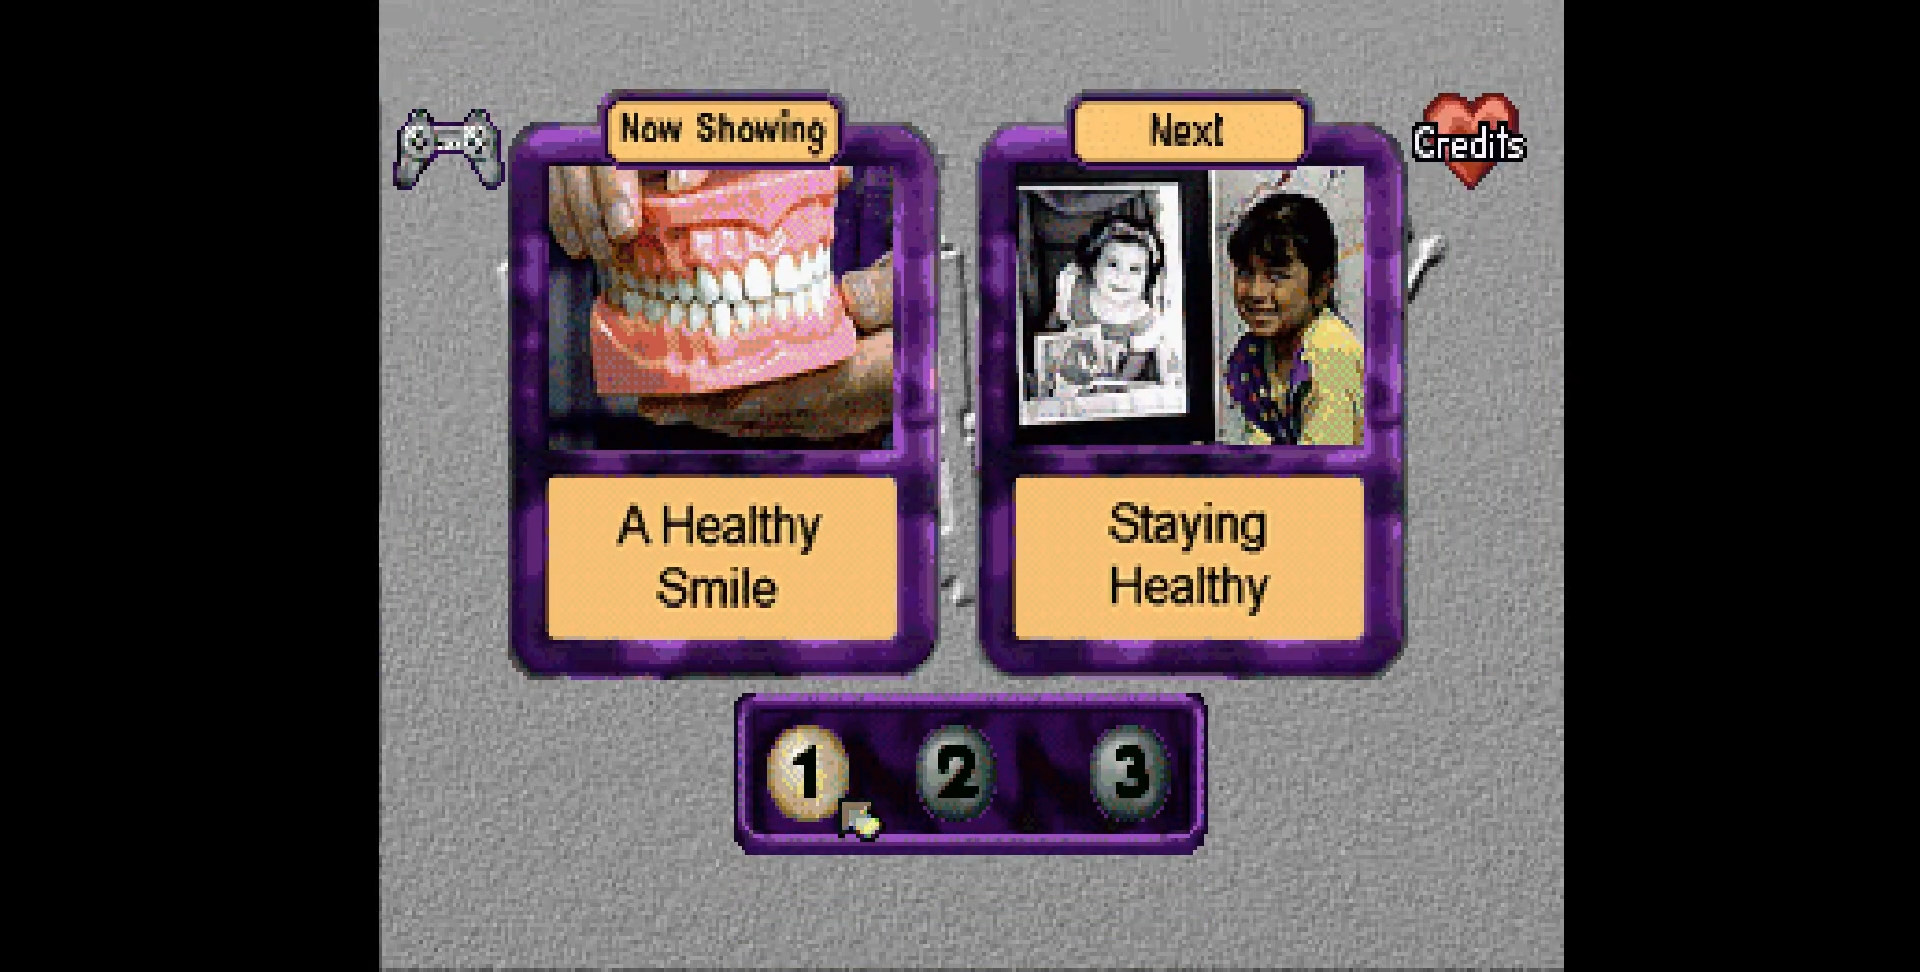
\includegraphics[width=\linewidth]{Games/HeadtoToe/Images/HeadToToe4Image1.png}
        \caption{Head To Toe 4 - Screenshot 1}
    \end{subfigure}
    \begin{subfigure}{0.45\textwidth}
        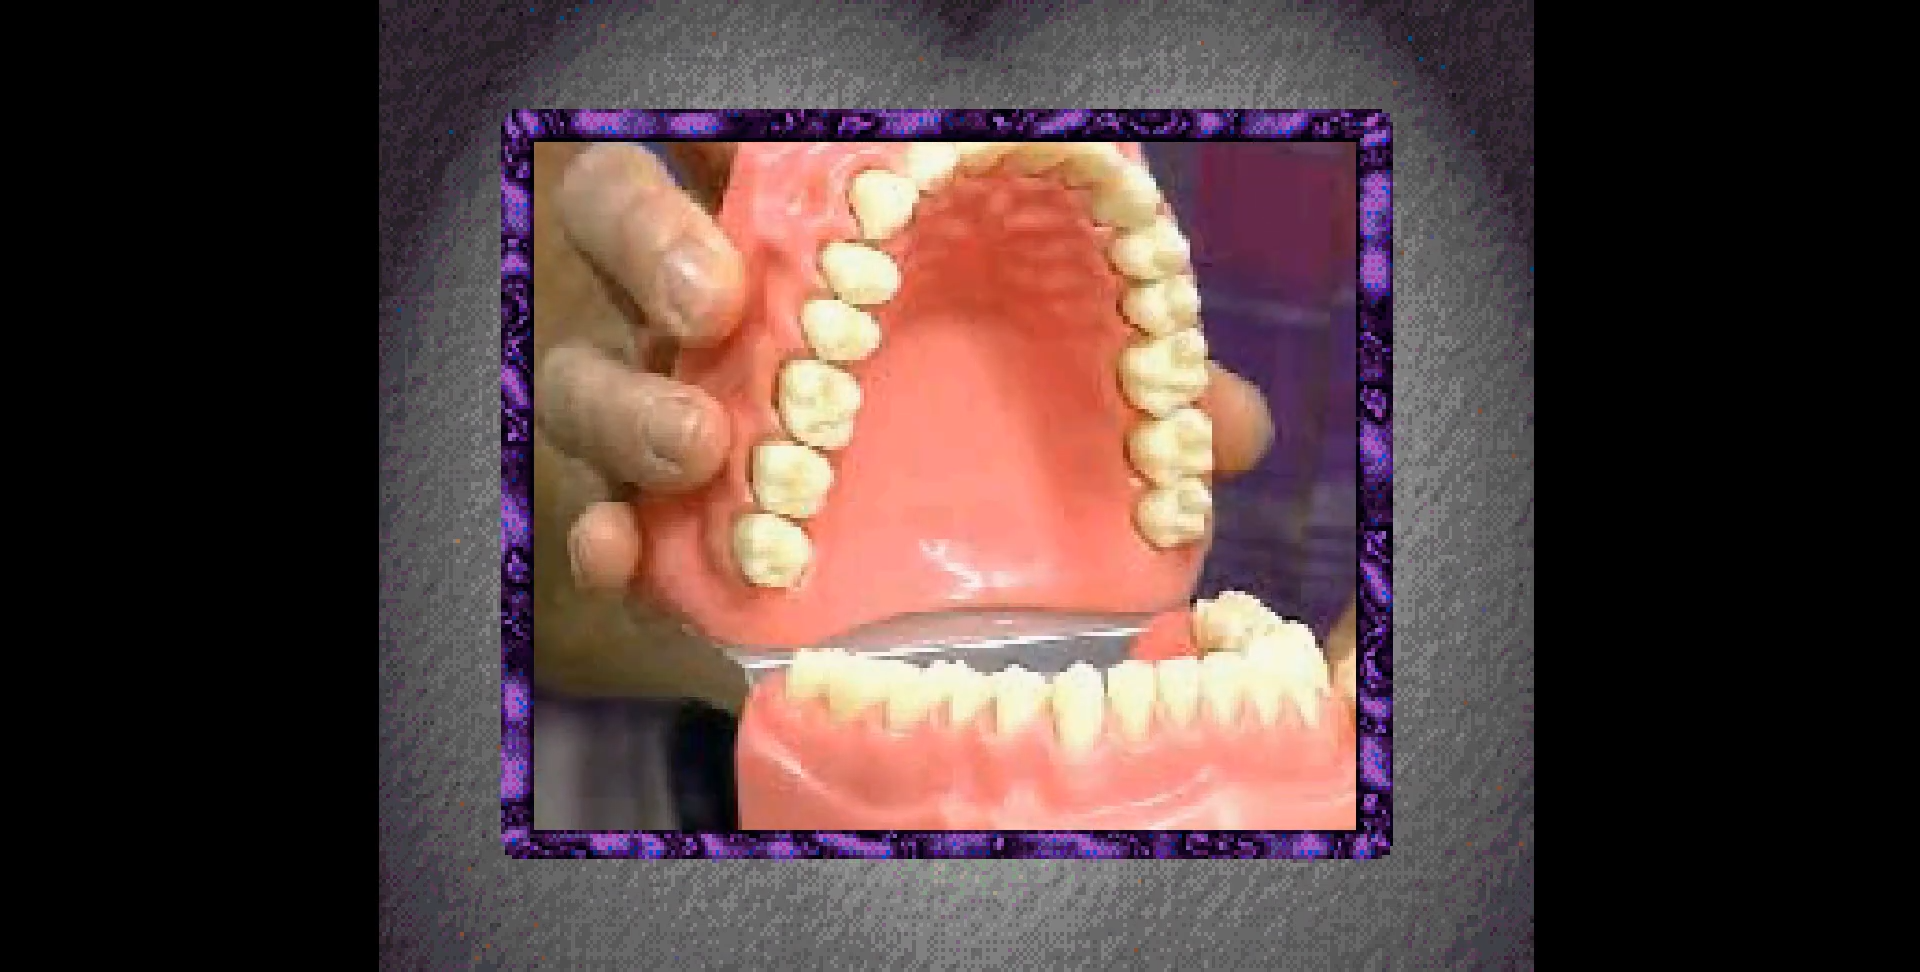
\includegraphics[width=\linewidth]{Games/HeadtoToe/Images/HeadToToe4Image2.png}
        \caption{Head To Toe 4 - Screenshot 2}
    \end{subfigure}

    \begin{subfigure}{0.45\textwidth}
        \centering
        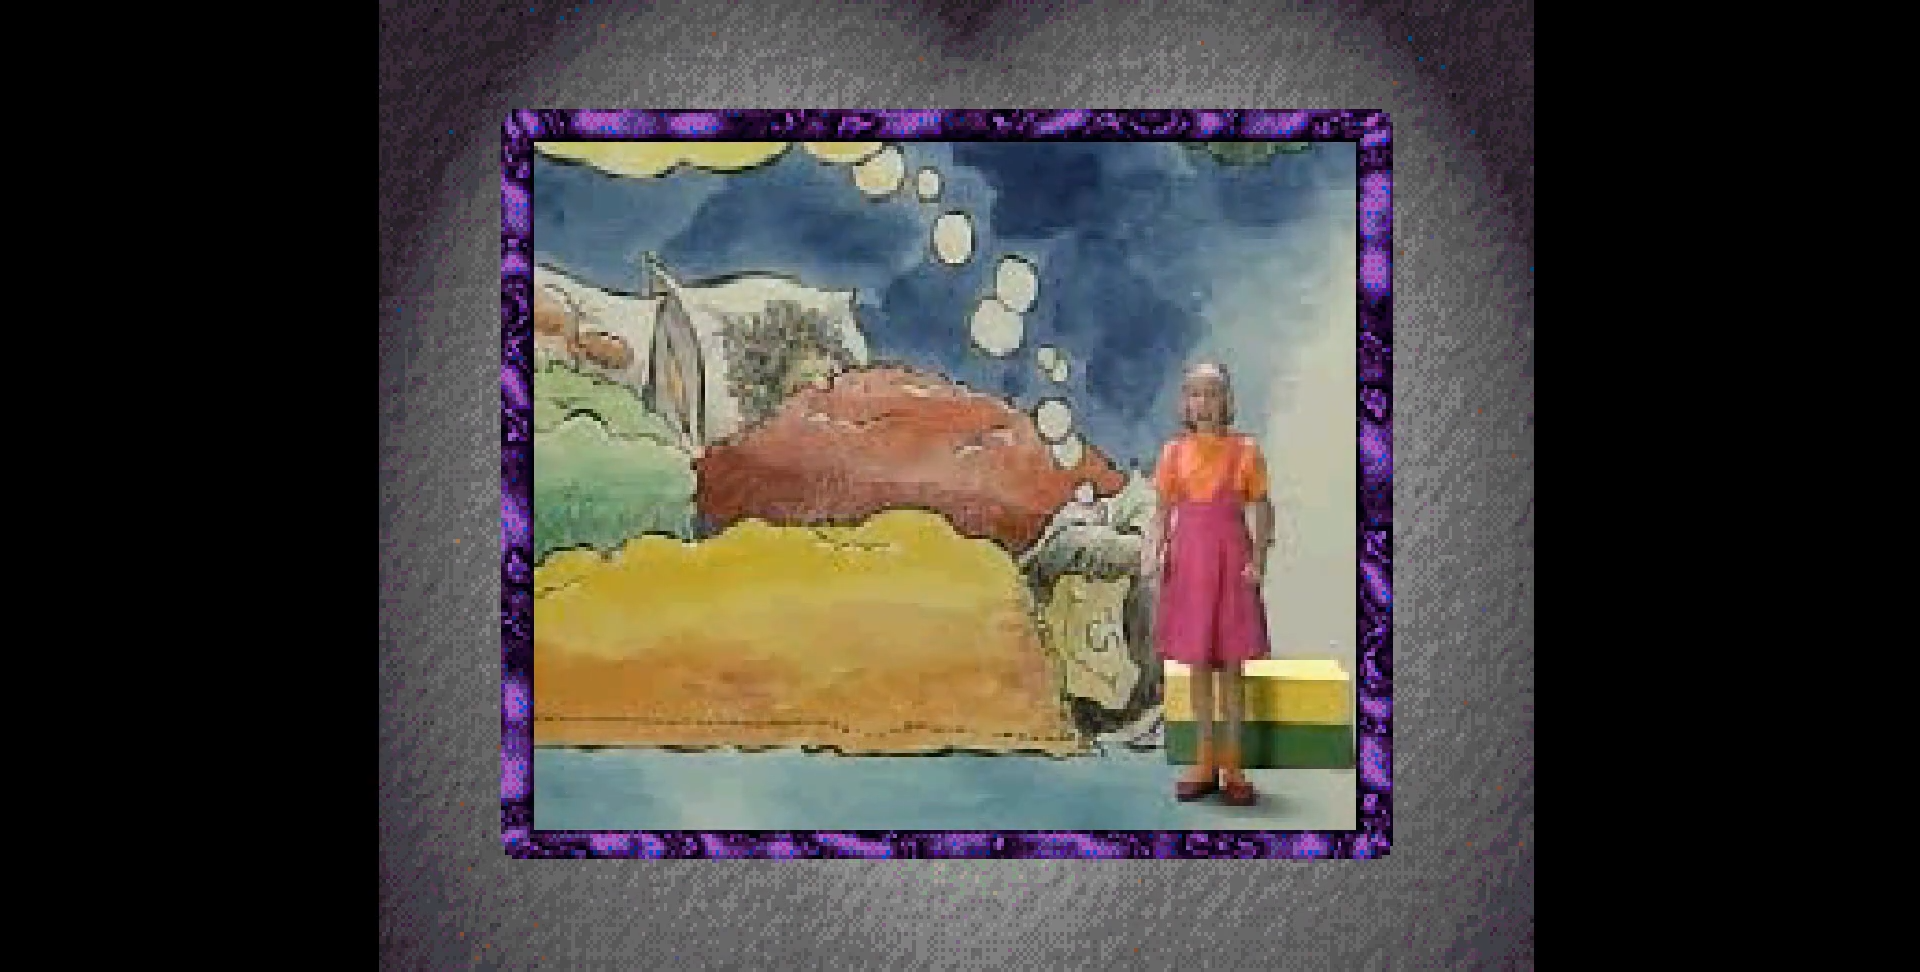
\includegraphics[width=\linewidth]{Games/HeadtoToe/Images/HeadToToe4Image3.png}
        \caption{Head To Toe 4 - Screenshot 3}
    \end{subfigure}
    \begin{subfigure}{0.45\textwidth}
        \centering
        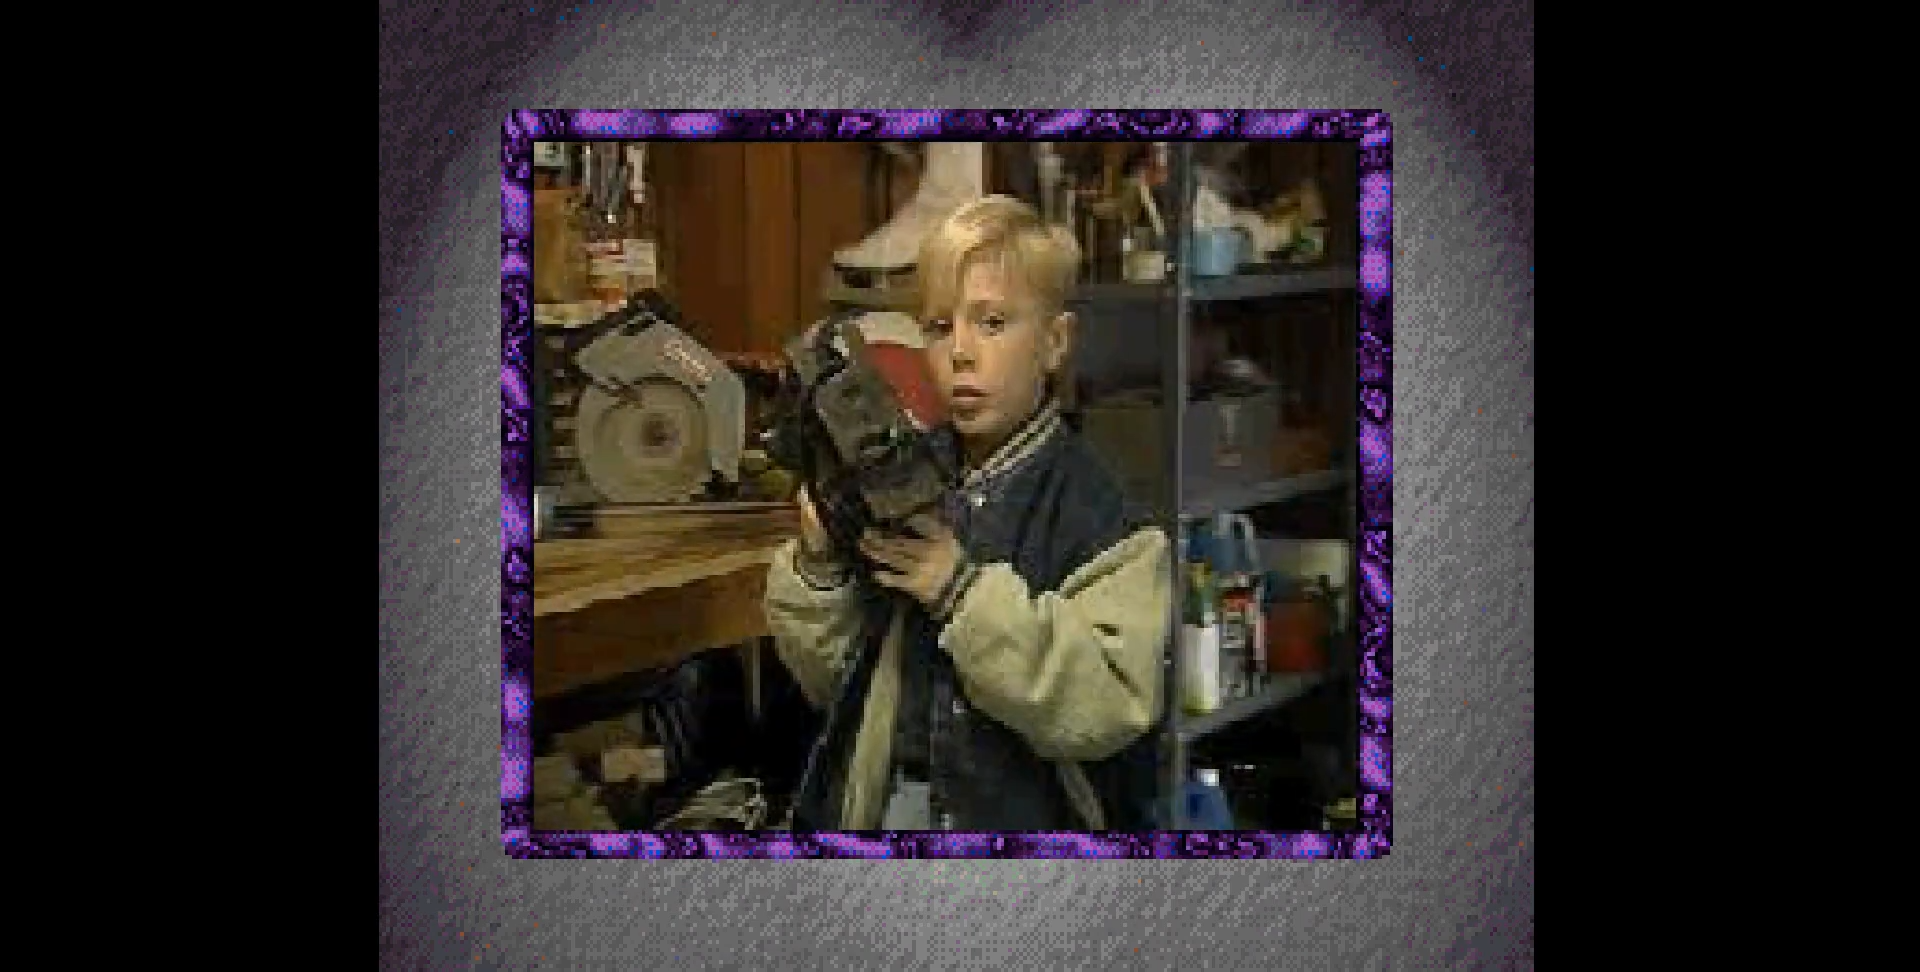
\includegraphics[width=\linewidth]{Games/HeadtoToe/Images/HeadToToe4Image4.png}
        \caption{Head To Toe 4 - Screenshot 4}
    \end{subfigure}
    \caption{Screenshots from Head To Toe 4}
\end{figure}